\pstart\noindent\hangindent=15mm\hspace{15mm}[21 v\textsuperscript{o}] Esto globus artificialis \textit{abc} in meridianos parallelosque subdivisus. Esto punctum discessus cognitum\edlabel{paralllend} \edtext{}{{\xxref{paralllstart}{paralllend}}\lemma{\textso{Parallelo.}}\Afootnote{ \textit{ (1) }\ Cum detur \textit{ (2) }\ Pyxide inclinatoria\protect\index{Sachverzeichnis}{pyxis!inclinatoria|textit} exacte subdivisa satisque grandi, detur \textit{(a)}\ minimum  de miliari in miliare inclinationis\protect\index{Sachverzeichnis}{inclinatio|textit} mutatio \textit{(b)}\ (minimum) inclinationis\protect\index{Sachverzeichnis}{inclinatio|textit} ac proinde mutatio \textit{ (3) }\  Detur primum \textso{punctum discessus} cognitum inque globo artificiali notatum esse. \textit{ (4) }\  Esto globus [...] cognitum \textit{ L}}} \textit{d} cadens in parallelum\protect\index{Sachverzeichnis}{circulus parallelus} \textit{ed} meridianum\protect\index{Sachverzeichnis}{meridianus} \textit{ac} Nave\protect\index{Sachverzeichnis}{navis} progrediente extra parallelum\protect\index{Sachverzeichnis}{circulus parallelus} \textit{ed}. Esto punctum observationis novae primum, quo scilicet incipit sentiri mutatio inclinationis\protect\index{Sachverzeichnis}{inclinatio} \textit{f} (quod tanto se offeret  citius, ac proinde omnia erunt tanto exactiora  quanto pyxis inclinatoria\protect\index{Sachverzeichnis}{pyxis!inclinatoria} erit grandior, magisque  subdivisa). Hujus puncti \textit{f} cum detur inclinatio\protect\index{Sachverzeichnis}{inclinatio}  ex Hypothesi, dabitur et parallelus\protect\index{Sachverzeichnis}{circulus parallelus}. Ponamus eum parallelum \protect\index{Sachverzeichnis}{circulus parallelus} esse \textit{gh}. Cadet ergo punctum \textit{f} in \textit{gh}. Sed ut praecise determinetur, quod punctum paralleli\protect\index{Sachverzeichnis}{circulus parallelus} sit \textit{f} nihil aliud sciri opus est, quam angulus quem linea \textit{df} \edtext{seu distantia puncti cogniti et quaesiti faciat ad parallelum \textit{ed} in puncto cognito}{\lemma{\textit{df}}\Afootnote{ \textit{ (1) }\ fecerit ad parallelum\protect\index{Sachverzeichnis}{circulus parallelus|textit} \textit{ed}  in puncto cognito \textit{ (2) }\ seu [...] cognito \textit{ L}}} \textit{d}. Determinato enim puncto \edtext{\textit{d} unius parallelae \textit{ed}}{\lemma{}\Afootnote{\textit{d} unius parallelae \textit{ed} \textit{ erg.} \textit{ L}}} ex quo ducitur  recta \edtext{\textit{df}}{\lemma{}\Afootnote{\textit{df} \textit{ erg.} \textit{ L}}} de parallela \edtext{\textit{ed}}{\lemma{}\Afootnote{\textit{ed} \textit{ erg.} \textit{ L}}} in parallelam \edtext{\textit{gh}}{\lemma{}\Afootnote{\textit{gh} \textit{ erg.} \textit{ L}}}, determinatoque angulo \edtext{\textit{fde}}{\lemma{}\Afootnote{\textit{fde} \textit{ erg.} \textit{ L}}}, determinabitur quoque punctum \edtext{\textit{f}}{\lemma{}\Afootnote{\textit{f} \textit{ erg.} \textit{ L}}} in quo secabit \edtext{\textit{df}}{\lemma{}\Afootnote{\textit{df} \textit{ erg.} \textit{ L}}} alteram parallelam \edtext{\textit{gh}.}{\lemma{}\Afootnote{\textit{gh}. \textit{ erg.} \textit{ L}}}\newline Angulus \textit{fde} ita determinabitur: Constat quem angulum linea motus navis\protect\index{Sachverzeichnis}{navis} ad punctum cognitum \textit{d} initio  fecerit, seu ad quam plagam mundi se direxerit.  Hanc lineam cursus si servat, servabitur angulus \textit{fde} ac proinde cognitum erit punctum \textit{f}. Si  mutat, demonstrabit acus magnetica\protect\index{Sachverzeichnis}{acus!magnetica} \edtext{(demtis declinationibus)}{\lemma{}\Afootnote{(demtis declinationibus) \textit{ erg.} \textit{ L}}} quantitatem flexus ac proinde anguli mutationem; ac proinde punctum \textit{f} quo linea cursus navis\protect\index{Sachverzeichnis}{navis} utcunque flexa, secat parallelum\protect\index{Sachverzeichnis}{circulus parallelus} \textit{gh}. Ponatur \edtext{similiter}{\lemma{}\Afootnote{similiter \textit{ erg.} \textit{ L}}} navis\protect\index{Sachverzeichnis}{navis} primo moveri \edtext{}{\lemma{}\Afootnote{moveri  \textbar\ recta \textit{ erg. u. gestr.}\ \textbar\ ex \textit{ L}}} ex \textit{d} in  \textit{i}, et postea  flecti ex \textit{i} in \textit{f}. Invenietur utique eadem methodo primum punctum \textit{i} inde invenietur quoque punctum \textit{f}. \edtext{Notabitur \textit{h} in [globo]\edtext{}{\Afootnote{puncto\textit{\ L \"{a}ndert Hrsg.}}} artificiali\protect\index{Sachverzeichnis}{globus!artificialis} atque ita totus in eo cursus navis\protect\index{Sachverzeichnis}{navis}, tanto accuratius delineabitur, quanto pyxis\protect\index{Sachverzeichnis}{pyxis} erit exactius subdivisa.}{\lemma{}\Afootnote{Notabitur \textit{h} in [globo]\edtext{}{\Afootnote{puncto\textit{\ L \"{a}ndert Hrsg.}}} artificiali\protect\index{Sachverzeichnis}{globus!artificialis} atque [...] subdivisa. \textit{ erg.} \textit{ L}}}  Dixi a flexu navis\protect\index{Sachverzeichnis}{navis} cognoscendo \hfill adimendas esse\pend
  \begin{center}
  %\begin{wrapfigure}{l}{0.7\textwidth}                    
  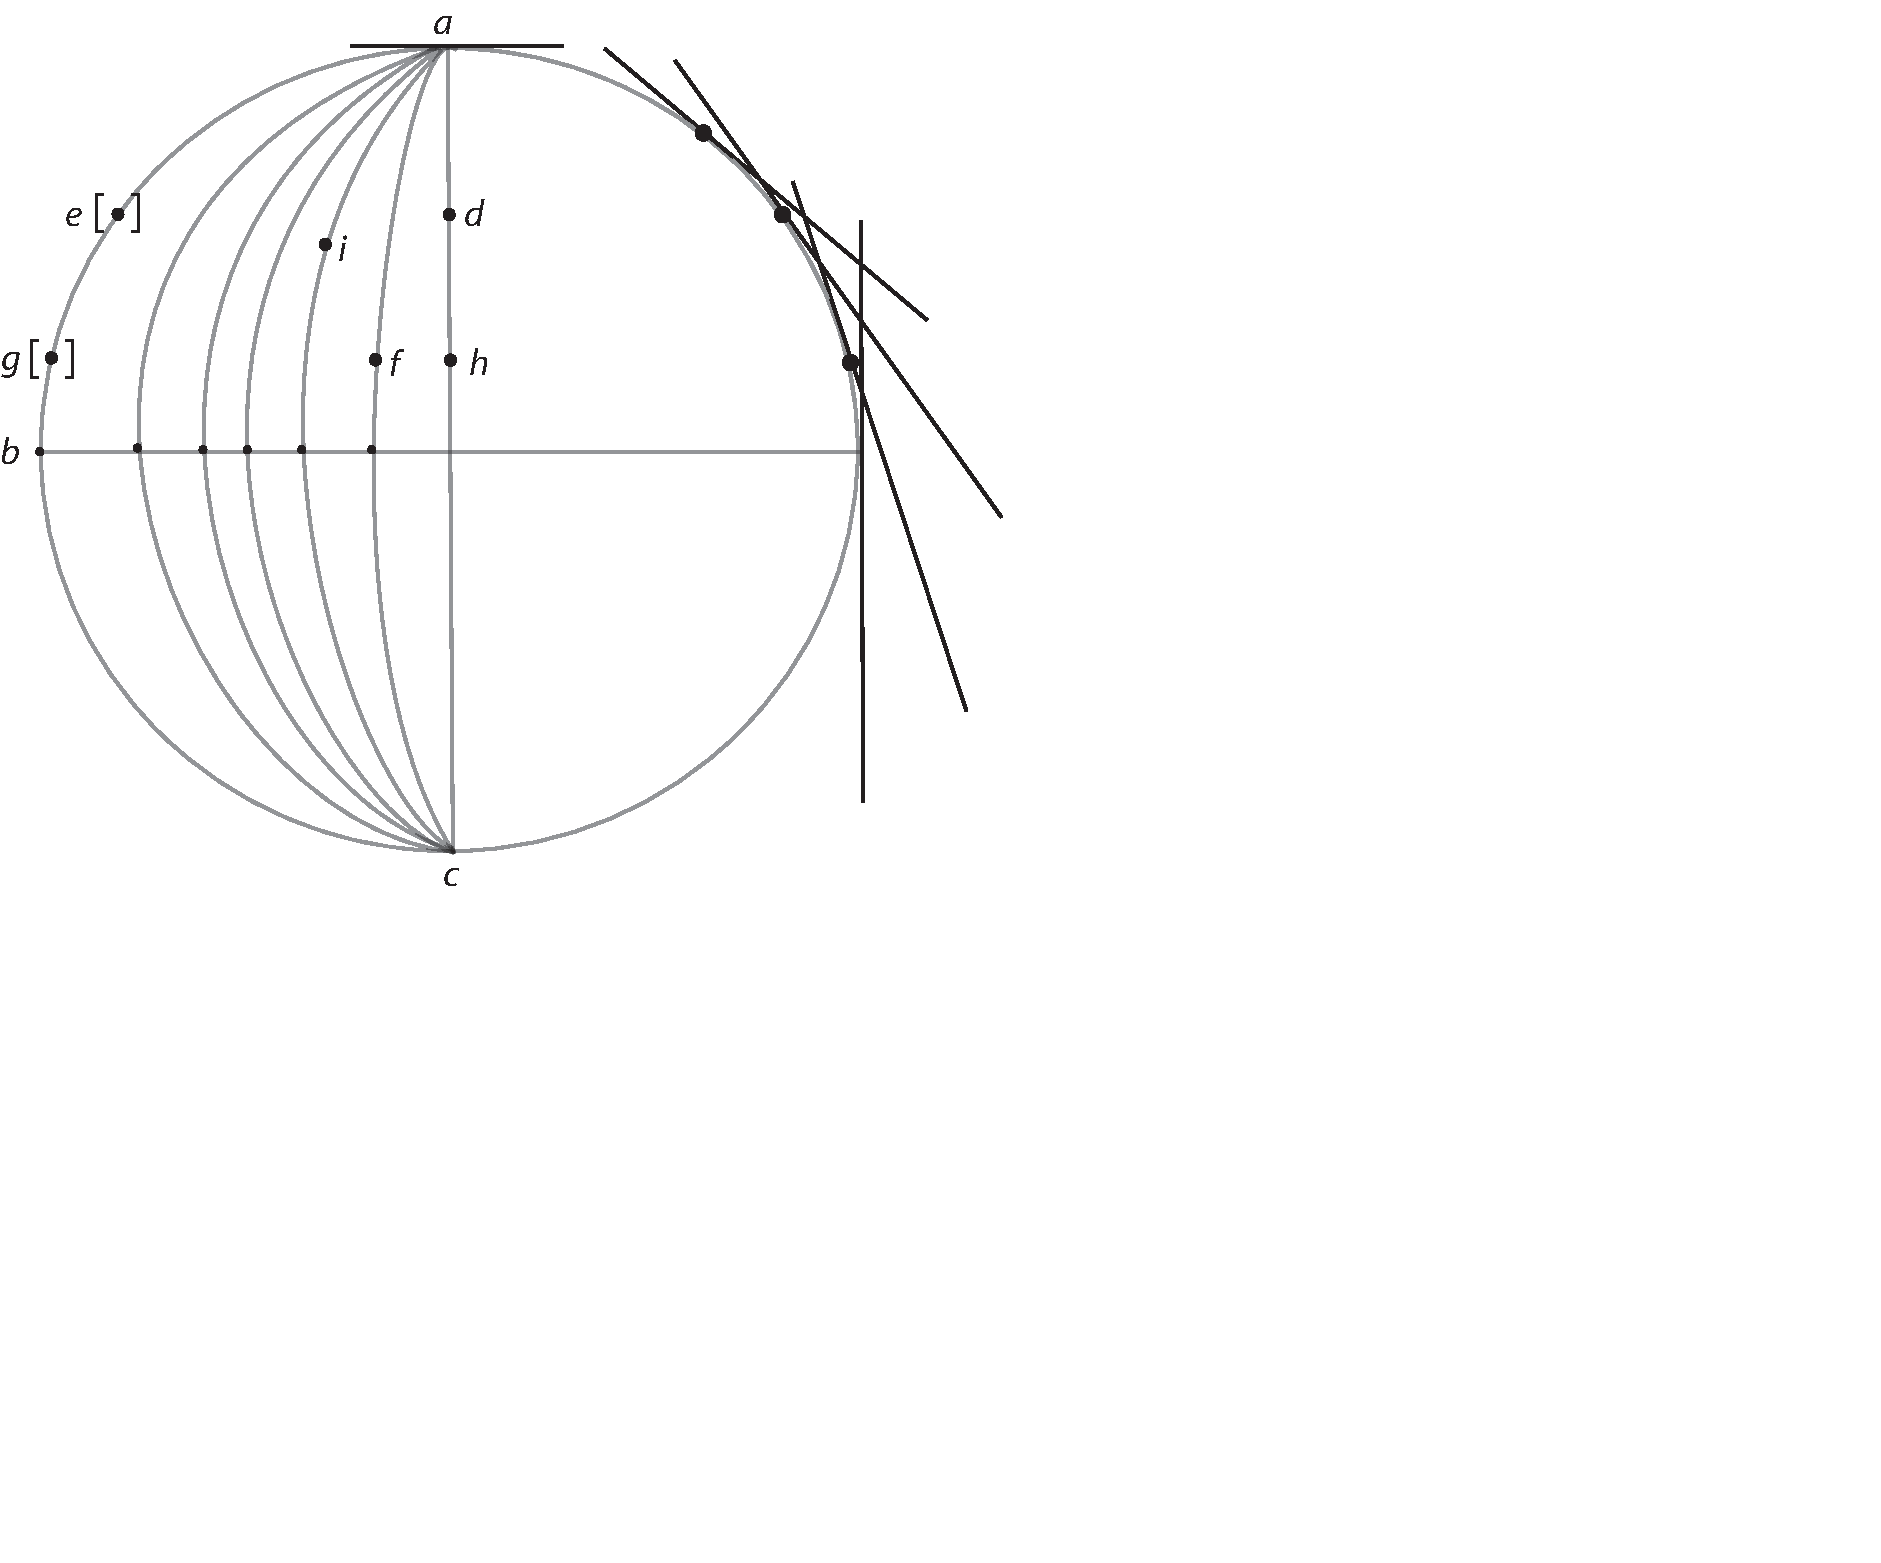
\includegraphics[width=0.9\textwidth]{images/38_21v}
 %\caption{Bildbeschreibung}
 \end{center}\begin{center}
  \textit{[Fig. 2, tlw. Blindzeichnung]}
  \end{center}
  %\end{wrapfigure}
\pstart\noindent\hangindent=15mm\hspace{15mm}magnetis\protect\index{Sachverzeichnis}{magnes} declinationes\protect\index{Sachverzeichnis}{declinatio}. \edtext{Hoc non habet magnas difficultates}{\lemma{declinationes.}\Afootnote{ \textit{ (1) }\ Esto ergo problema. \textit{ (2) }\   (4) \textso{Magnetis}\protect\index{Sachverzeichnis}{magnes|textit}\textso{ }\textso{declinationes}\protect\index{Sachverzeichnis}{declinatio|textit}\textso{ invenire} \textit{ (3) }\ Hoc  \textit{(a)}\ problema communi quoque via \textit{(b)}\ non  \textit{(aa)}\ est magnae difficultatis \textit{(bb)}\ habet magnas difficultates \textit{ L}}}, notari enim potest in longissimis etiam itineribus in Indiam\protect\index{Ortsregister}{Indien (India)} orientalem susceptis, nautas pene quotidie, ut eorum diaria monstrant, observandarum declinationum\protect\index{Sachverzeichnis}{declinatio} potestatem \edtext{habuisse. Quod ut exacte fiat an}{\lemma{habuisse.}\Afootnote{ \textit{ (1) }\ Sed si verum  est dari in magnete\protect\index{Sachverzeichnis}{magnes|textit} aut acu\protect\index{Sachverzeichnis}{acus!magnetica|textit}  \textit{(a)}\ verticali \textit{(b)}\ Meridianum\protect\index{Sachverzeichnis}{meridianus|textit} universalem sine declinatione\protect\index{Sachverzeichnis}{declinatio|textit}, quod valde  \textit{(aa)}\ observo \textit{(bb)}\ operae pretium est experimento comprobari,  sine omni observatione declinationes\protect\index{Sachverzeichnis}{declinatio|textit} habebuntur. Et inventum hoc ad  summam perfectionem optabilem  \textit{(aaa)}\ perfectum \textit{(bbb)}\ provectum erit. \textit{ (2) }\ Quod ut exacte fiat an \textit{ L}}} [\textit{Satz bricht ab}]\footnote{\textit{Auf Blatt 21 v\textsuperscript{o} am oberen Rand}: (+ NB ista non procedunt. Nisi constet distantia inter quemlibet novum flexum. Alioqui non datur linea motus navis, sed tantum ei parallela. +)} \pend \pstart\noindent\hangindent=15mm  (5) \textso{Locum }\textso{navis}\protect\index{Sachverzeichnis}{navis}\textso{ invenire.} Invento cursu navis\protect\index{Sachverzeichnis}{navis} per probl. 3. \edtext{inventus}{\lemma{probl. 3.}\Afootnote{ \textit{ (1) }\ datus \textit{ (2) }\ inventus \textit{ L}}} erit quoque locus navis\protect\index{Sachverzeichnis}{navis}, quippe  extremum cursus tempore dato. Loco navis\protect\index{Sachverzeichnis}{navis} invento,  solutum est magnum hoc problema.\pend \pstart\noindent\hangindent=15mm  (6) \textso{Longitudines}\protect\index{Sachverzeichnis}{longitudo}\textso{ }\edtext{\textso{invenire}}{\lemma{\textso{Longitudines}}\Afootnote{ \textit{ (1) }\ \textso{observare} \textit{ (2) }\ \textso{invenire} \textit{ L}}}\textso{, }\edtext{\textso{declinationibus tantum}}{\lemma{\textso{invenire,}}\Afootnote{ \textit{ (1) }\ \textso{solis} \textit{ (2) }\ \textso{declinationibus tantum} \textit{ L}}}\textso{ }\textso{magneticis}\textso{ }\protect\index{Sachverzeichnis}{magnes}\textso{ observatis.} Nulla licet Theoria seu Regula \edtext{Universali declinationum}{\lemma{Universali}\Afootnote{ \textit{ (1) }\ Latitudinum\protect\index{Sachverzeichnis}{latitudo|textit} \textit{ (2) }\ declinationum \textit{ L}}} constituta.\newline Multi hactenus ex declinationibus\protect\index{Sachverzeichnis}{declinatio} longitudines\protect\index{Sachverzeichnis}{longitudo} promisere, sed \edtext{vel}{\lemma{sed}\Afootnote{ \textit{ (1) }\ quia \textit{ (2) }\ vel \textit{ L}}} theoriam quandam universalem declinationum\protect\index{Sachverzeichnis}{declinatio}  quae tamen falsa comperta est, vel aliorum observationes  de declinationibus\protect\index{Sachverzeichnis}{declinatio} supposuere quae tamen tractu temporis  immutatae \edtext{sunt}{\lemma{immutatae}\Afootnote{ \textit{ (1) }\ fecere \textit{ (2) }\ sunt \textit{ L}}}. Hic vero nulla theoria, \edtext{nullis diversis observationibus}{\lemma{theoria,}\Afootnote{ \textit{ (1) }\ nulla diversorum  temporum locorumque observatione \textit{ (2) }\ nullis diversis observationibus \textit{ L}}}, sed sola diligenti in eadem navi\protect\index{Sachverzeichnis}{navis} repetita subinde declinationum observatione opus est. Quam alioqui a bonis Navium\protect\index{Sachverzeichnis}{navis} rectoribus semper fieri debere constat.\pend
